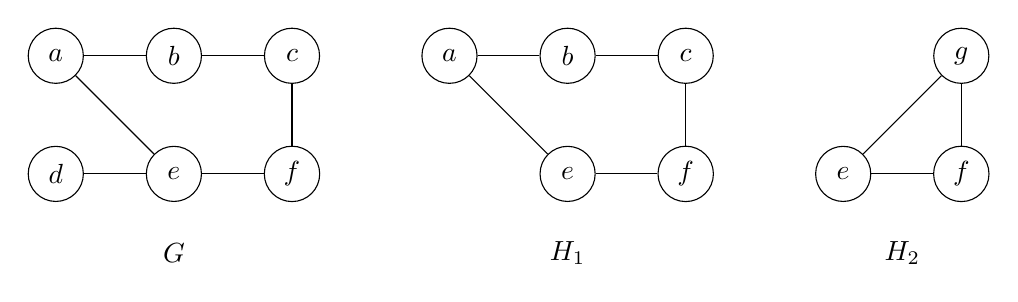
\begin{tikzpicture}

\node [circle, minimum height=0.7cm, draw] (v1) at (0,0) {$a$};
\node [circle, minimum height=0.7cm, draw] (v2) at (1.5,0) {$b$};
\node [circle, minimum height=0.7cm, draw] (v3) at (3,0) {$c$};
\node [circle, minimum height=0.7cm, draw] (v4) at (3,-1.5) {$f$};
\node [circle, minimum height=0.7cm, draw] (v5) at (1.5,-1.5) {$e$};
\node [circle, minimum height=0.7cm, draw] (v6) at (0,-1.5) {$d$};
\draw  (v1) edge (v2);
\draw  (v2) edge (v3);
\draw  (v3) edge (v4);
\draw  (v4) edge (v5);
\draw  (v5) edge (v1);
\draw  (v5) edge (v6);

\node [circle, minimum height=0.7cm, draw] (v12) at (5,0) {$a$};
\node [circle, minimum height=0.7cm, draw] (v13) at (6.5,0) {$b$};
\node [circle, minimum height=0.7cm, draw] (v14) at (8,0) {$c$};
\node [circle, minimum height=0.7cm, draw] (v15) at (8,-1.5) {$f$};
\node [circle, minimum height=0.7cm, draw] (v16) at (6.5,-1.5) {$e$};
\draw  (v12) edge (v13);
\draw  (v13) edge (v14);
\draw  (v14) edge (v15);
\draw  (v15) edge (v16);
\draw  (v16) edge (v12);

\node [circle, minimum height=0.7cm, draw] (v7) at (11.5,0) {$g$};
\node [circle, minimum height=0.7cm, draw] (v8) at (11.5,-1.5) {$f$};
\node [circle, minimum height=0.7cm, draw] (v9) at (10,-1.5) {$e$};
\draw  (v7) edge (v8);
\draw  (v8) edge (v9);
\draw  (v9) edge (v7);


\node [] at (1.5,-2.5) {$G$};
\node [] at (6.5,-2.5) {$H_1$};
\node [] at (10.75,-2.5) {$H_2$};
\end{tikzpicture}